\documentclass[border={-5pt -5pt -5pt -3pt}]{standalone}

\usepackage{hyperref}
\usepackage{tikz}

\usetikzlibrary{decorations.pathreplacing,
  arrows,
  calc,
  decorations.pathmorphing,
  decorations.pathreplacing,
  decorations.markings,
  fadings,
  positioning,
  shapes,
  3d
}

\ifpdf
% Ensure reproducible output
\pdfinfoomitdate=1
\pdfsuppressptexinfo=-1
\pdftrailerid{}
\hypersetup{
  pdfcreator={},
  pdfproducer={}
}
\fi

\begin{document}
\begin{tikzpicture}
  \node at (0, 0 + 4.5 * 2) {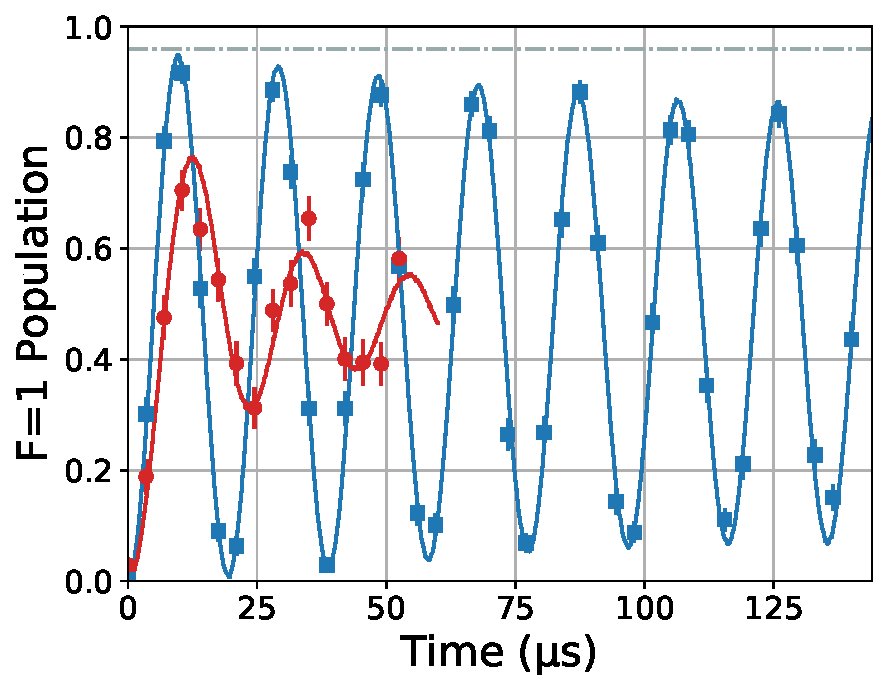
\includegraphics[height=4.5cm]{na_rsc_rabi_flop_rx_0.pdf}};
  \node at (6.0, 0 + 4.5 * 2) {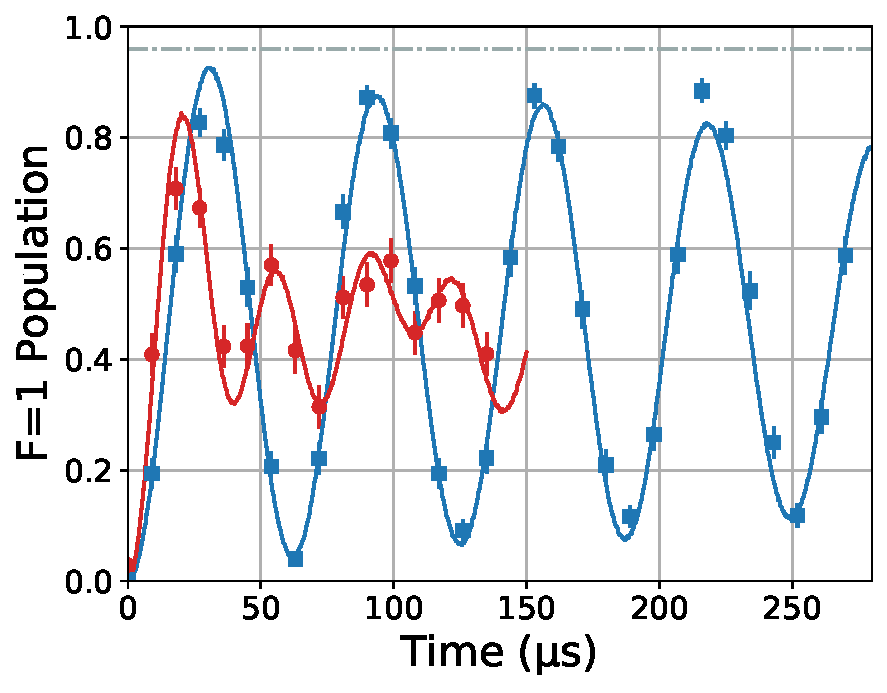
\includegraphics[height=4.5cm]{na_rsc_rabi_flop_rx_p1.pdf}};
  \node at (2.5, 1.7 + 4.5 * 2) {\scriptsize (\textbf{A})};
  \node at (8.52, 1.7 + 4.5 * 2) {\scriptsize (\textbf{B})};
  \node at (0, 0 + 4.5) {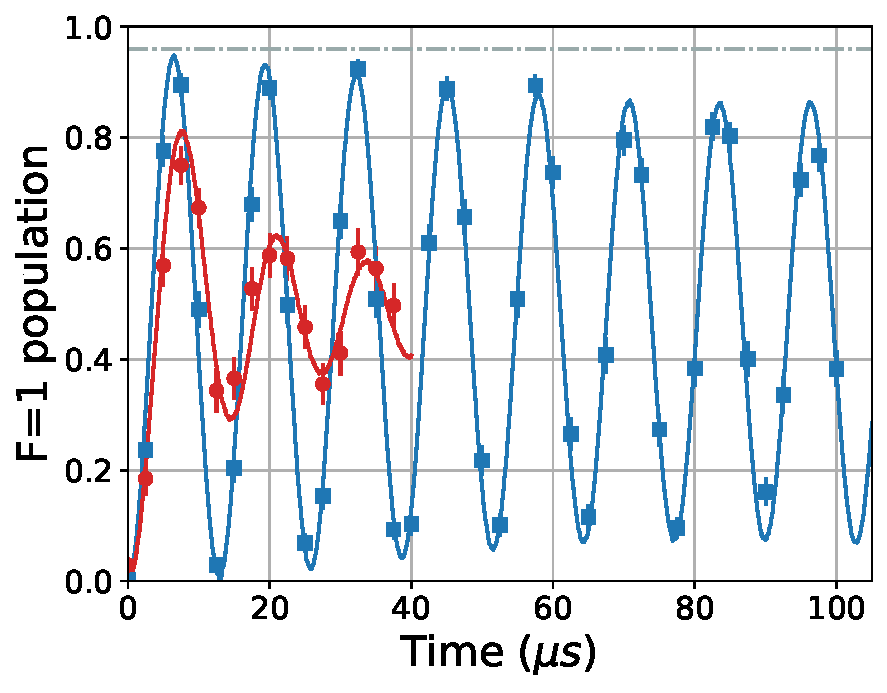
\includegraphics[height=4.5cm]{na_rsc_rabi_flop_ry_0.pdf}};
  \node at (6.0, 0 + 4.5) {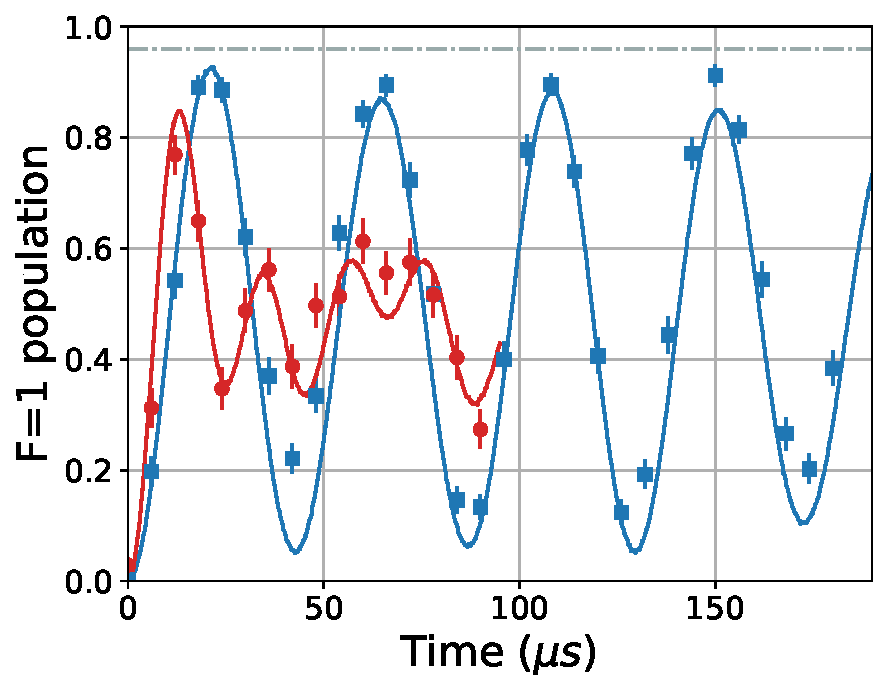
\includegraphics[height=4.5cm]{na_rsc_rabi_flop_ry_p1.pdf}};
  \node at (2.5, 1.75 + 4.5) {\scriptsize (\textbf{C})};
  \node at (8.42, 1.65 + 4.5) {\scriptsize (\textbf{D})};
  \node at (0, 0) {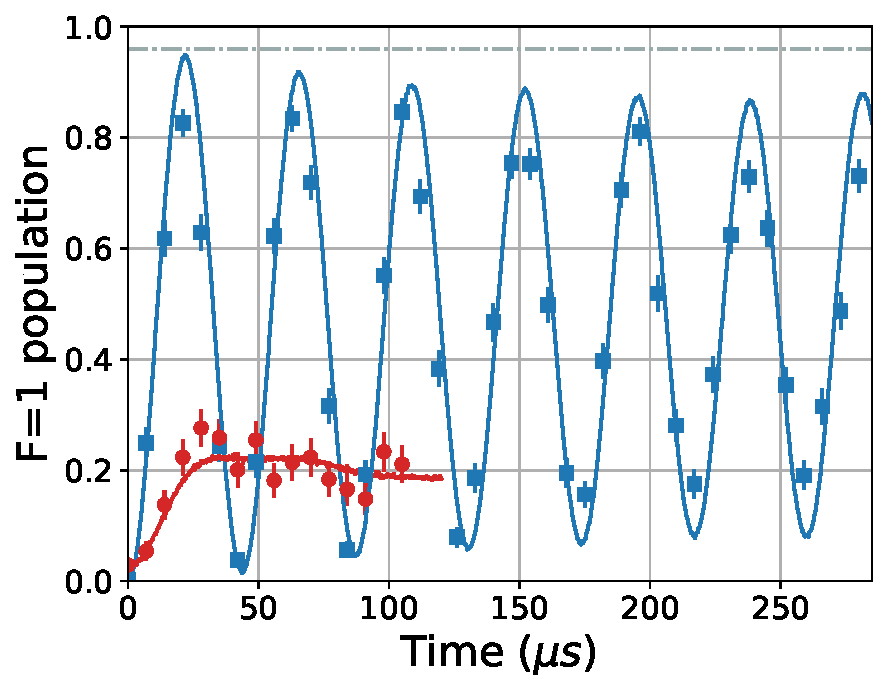
\includegraphics[height=4.5cm]{na_rsc_rabi_flop_az_0.pdf}};
  \node at (6.0, 0) {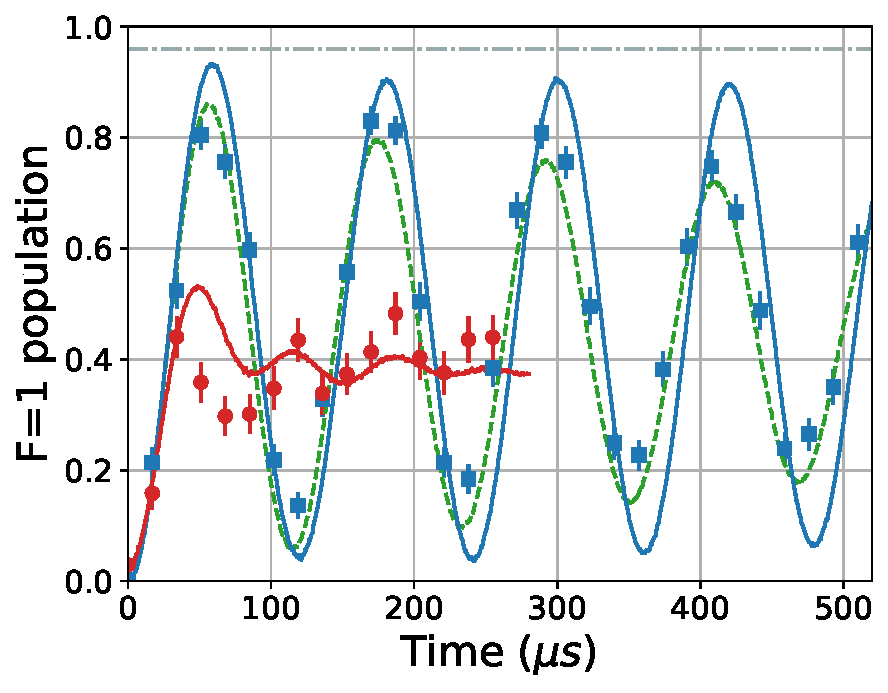
\includegraphics[height=4.5cm]{na_rsc_rabi_flop_az_p1.pdf}};
  \node at (2.45, 1.7) {\scriptsize (\textbf{E})};
  \node at (8.35, 1.7) {\scriptsize (\textbf{F})};
\end{tikzpicture}
\end{document}
